\documentclass[a4paper,fontset = windowsnew]{ctexart}
\usepackage[margin=2cm]{geometry}
\usepackage{xifthen}
\usepackage{calc}
\usepackage{graphicx}
%\usepackage{tikz}
%\usepackage{amsmath}
\usepackage[user=student]{cexam}
%\usepackage[user=teacher]{cexam}
\usepackage[
  pdfborder=0 0 0,
  bookmarksnumbered=true
]{hyperref}

\begin{document}
%\ExplSyntaxOn
%\bool_set_true:N \answer_student_bool
%\iow_open:Nn \answer_write {\jobname.ans}
%\ExplSyntaxOff

%\chapter{试题排版环境测试}

\section{各题型测试}

%\parindent=0pt

\begin{choices}
  1.这是选择题的题干,如
  <<
  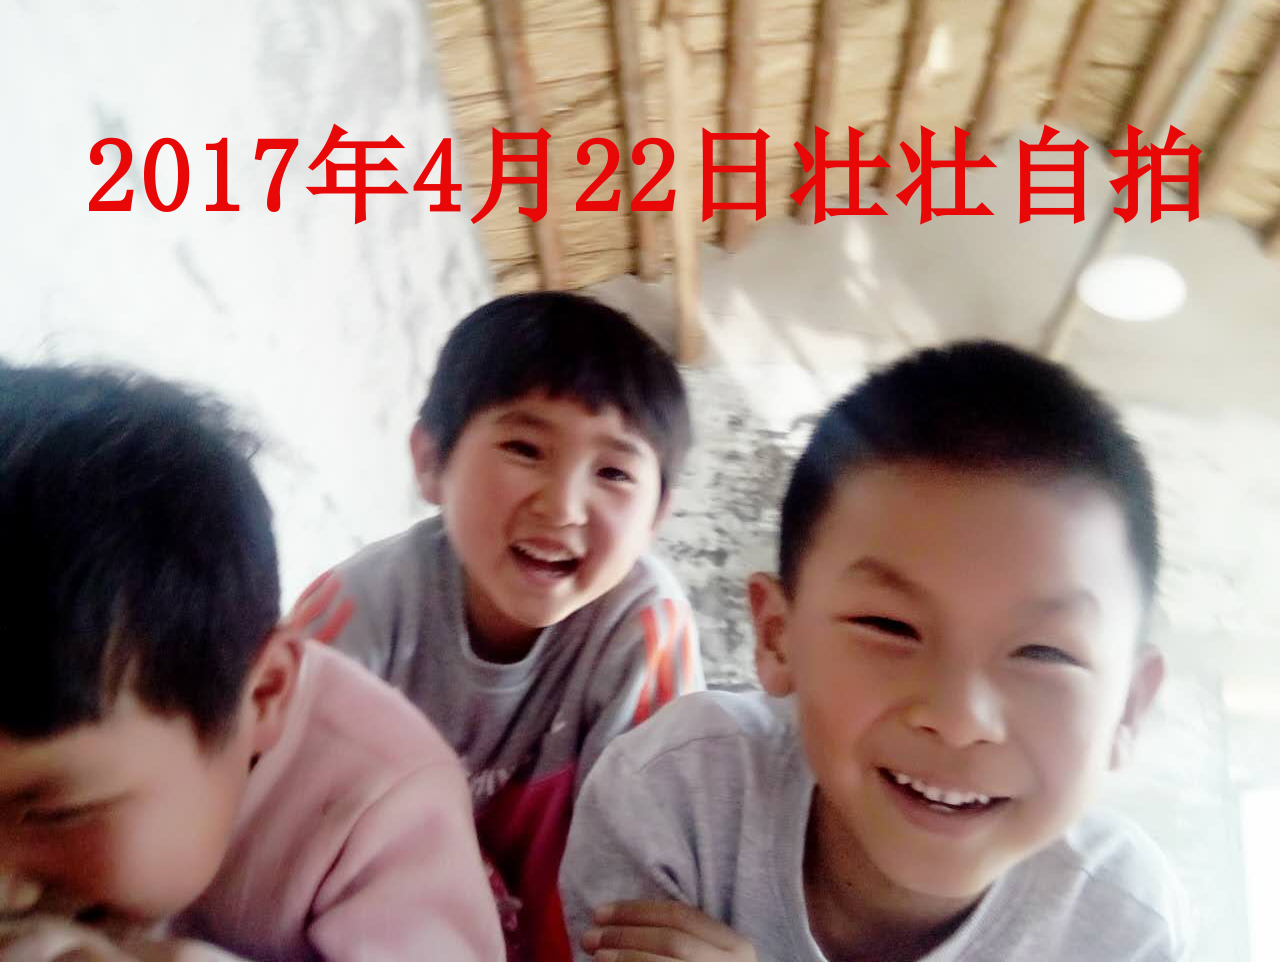
\includegraphics[scale=0.2]{2.jpg}
  >>
  所示是图片.其中有四个选项,分别是
  A.选项A
  B.选项B
  C.选项C
  D.选项D

  a.AB

  e.这是选择题的解析部分.

  ee.这是选择题解析下一级部分,用来输入解析较长的情况.

  1.这是选择题的题干,如
  <<
  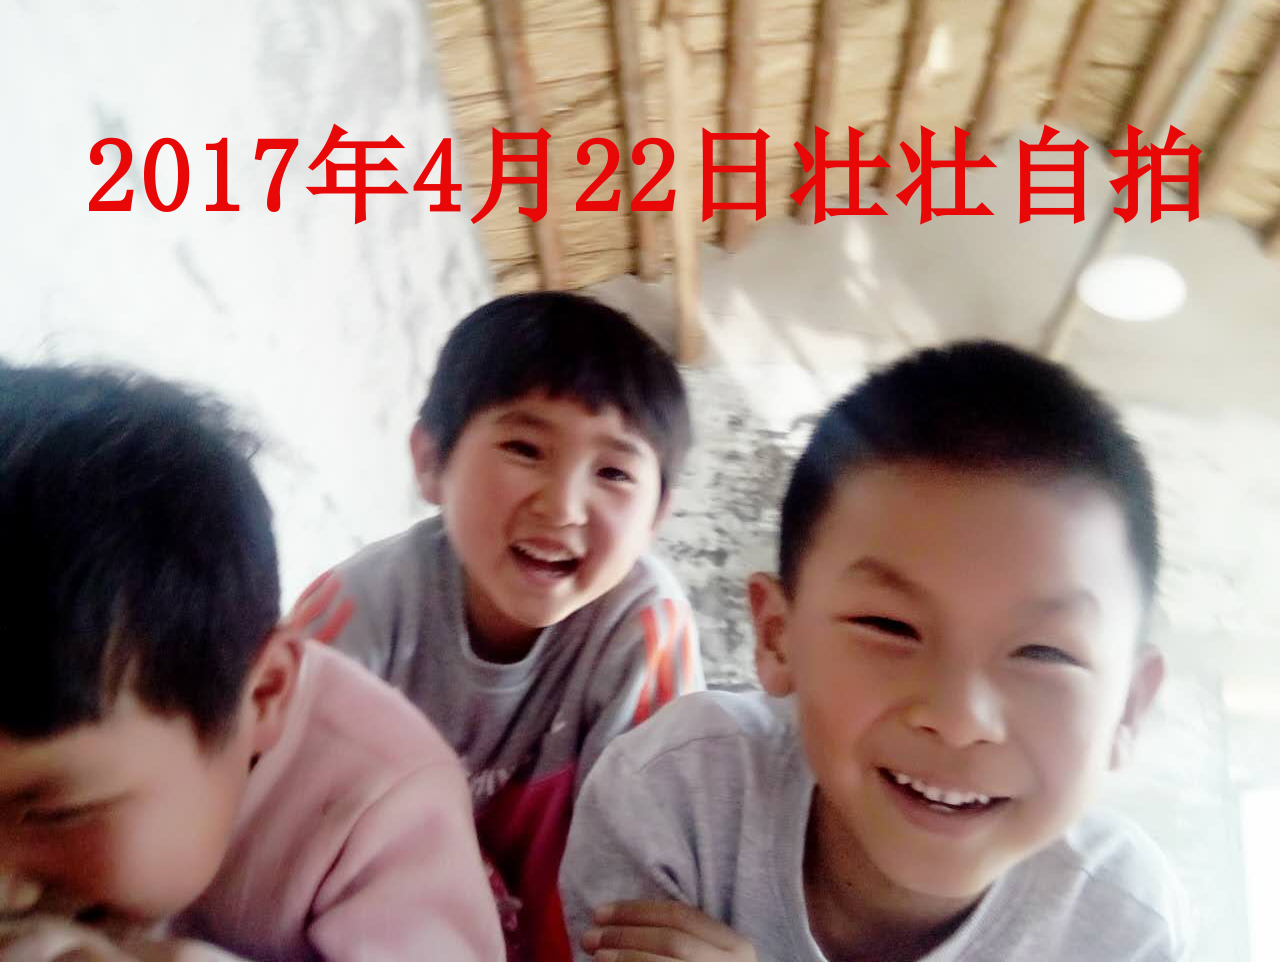
\includegraphics[scale=0.15]{2.jpg}
  >>
  所示是图片.其中有四个选项,分别是
  所示是图片.其中有四个选项,分别是
  所示是图片.其中有四个选项,分别是
  所示是图片.其中有四个选项,分别是
  所示是图片.其中有四个选项,分别是
  A.选项A选项A选项A选项A选项A
  B.选项B选项B选项B
  C.选项C
  D.选项D

  a.ABCD

  e.这是第二题的解析.
  <<
  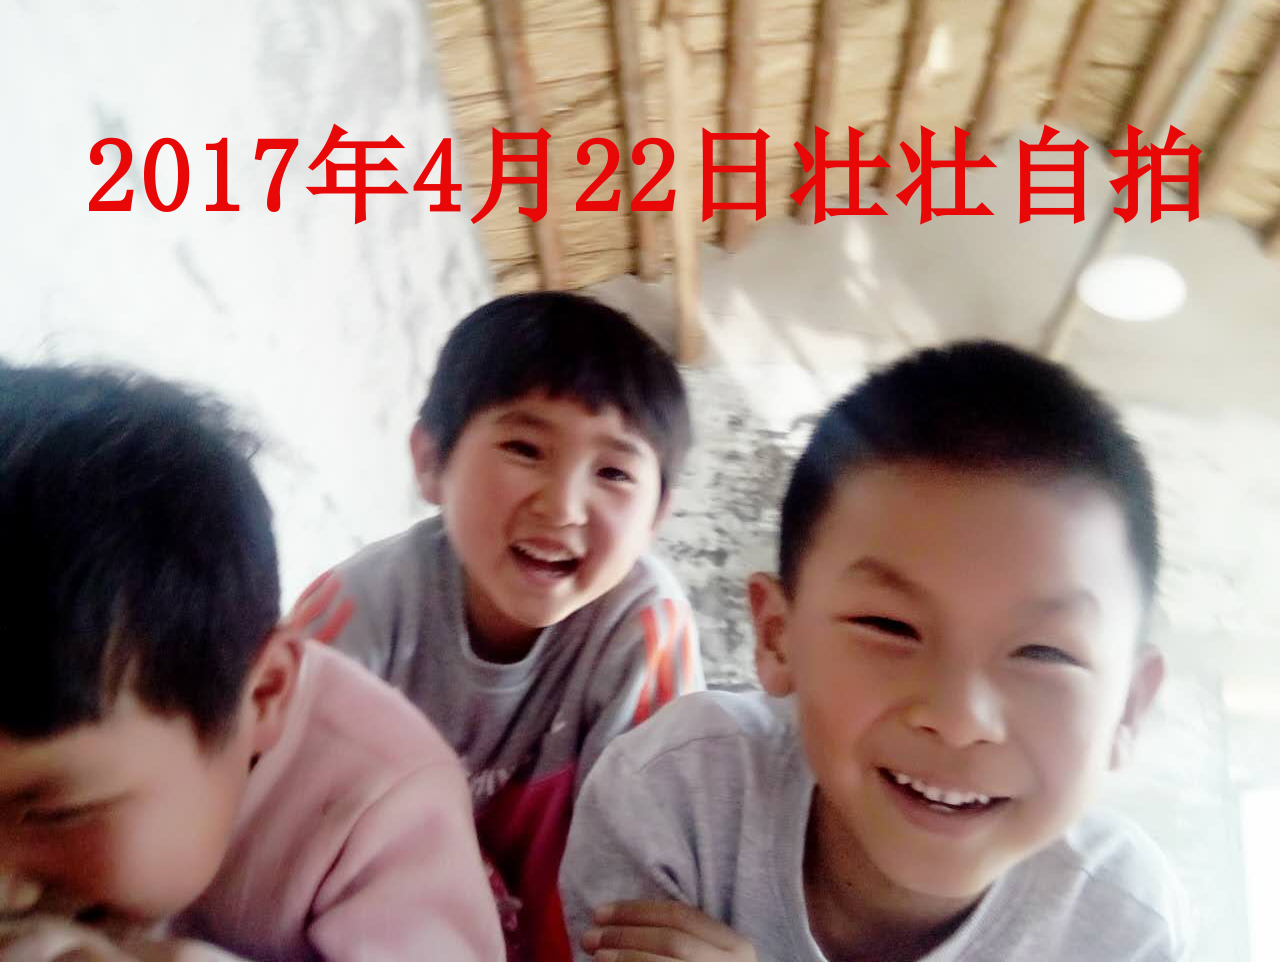
\includegraphics[scale=0.2]{2.jpg}
  >>
  所示是图片.其中有四个选项,分别是
  所示是图片.其中有四个选项,分别是
  所示是图片.其中有四个选项,分别是
  所示是图片.其中有四个选项,分别是
  所示是图片.其中有四个选项,分别是
  所示是图片.其中有四个选项,分别是
  所示是图片.其中有四个选项,分别是

  ee.这是第二题的追加解析.

  1.这是选择题的题干,如
  <<
  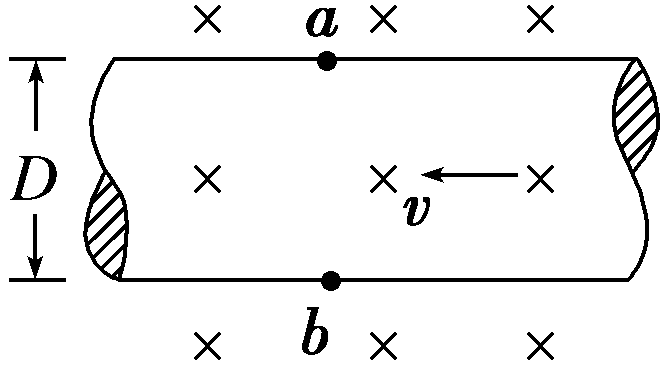
\includegraphics{1.png}
  >>
  所示是图片.其中有四个选项,分别是
  所示是图片.其中有四个选项,分别是
  所示是图片.其中有四个选项,分别是
  所示是图片.其中有四个选项,分别是
  所示是图片.其中有四个选项,分别是
  A.选项A
  B.选项B
  C.选项C
  D.选项D

\end{choices}

这是输入选择题后的测试文本缩进的文字.
这是输入选择题后的测试文本缩进的文字.
这是输入选择题后的测试文本缩进的文字.
这是输入选择题后的测试文本缩进的文字.
这是输入选择题后的测试文本缩进的文字.
\newpage
\begin{blanks}
1.这是计算题的题干
这是\blank{计算题}的题干这是计算题的题干
\begin{equation}
  E=MC^2
\end{equation}
这是计算题的题干这是\blank{计算题}的题干
<<
\begin{tikzpicture}
  \draw (0,0) rectangle (5,3);
\end{tikzpicture}
>>
这是计算题的\blank{题干}这是计算题的\blank{题干}
这是计算题的题干这是计算题的题干

a.*

e.这是填空题的解析部分.用以测试填空题解析输出.

ee.这是填空题的追加解析部分.用以测试填空题追加的解析输出.

1.这是计算题的题干
这是计算题的题干这是计算题的题干
\begin{equation}
  E=MC^2
\end{equation}
这是计算题的题干这是计算题的题干
<<
\begin{tikzpicture}
  \draw (0,0) rectangle (3,2);
\end{tikzpicture}
>>
这是计算题的题干这是计算题的题干
这是计算题的题干这是计算题的题干
这是计算题的题干这是计算题的题干
这是计算题的题干这是计算题的题干
这是计算题的题干这是计算题的题干
这是计算题的题干这是计算题的题干
这是计算题的题干这是计算题的题干
这是计算题的题干这是计算题的题干
这是计算题的题干这是计算题的题干
  
1.这是计算题的题干
这是计算题的题干这是计算题的题干
\begin{equation}
  E=MC^2
\end{equation}
这是计算题的题干这是计算题的题干
<<
\begin{tikzpicture}
  \draw (0,0) rectangle (3,3);
\end{tikzpicture}
>>
这是计算题的题干这是计算题的题干
这是计算题的题干这是计算题的题干

\end{blanks}


\newpage

\begin{judgements}
  1.这是判断题的输出测试,用来排版判断题.

  a.对

1.这是计算题的题干
这是计算题的题干这是计算题的题干
\begin{equation}
  E=MC^2
\end{equation}
这是计算题的题干这是计算题的题干
<<
\begin{tikzpicture}
  \draw (0,0) rectangle (3,3);
\end{tikzpicture}
>>
这是计算题的题干这是计算题的题干
这是计算题的题干这是计算题的题干

a.错

e.这是判断题的解析.2019年9月3日晚完成了全部内容.

\end{judgements}

\begin{calculations}
  1.这是计算题的输出测试,用来排版计算题.

  a.这是计算题的答案.它是第一题的答案测试.

e.这是计算题的解析.2019年9月17日晚完成了全部内容.

1.这是计算题的题干
这是计算题的题干这是计算题的题干
%\begin{equation}
\[  E=MC^2 \]
%\end{equation}
这是计算题的题干这是计算题的题干
<<
\begin{tikzpicture}
  \draw (0,0) rectangle (3,2);
\end{tikzpicture}
>>
这是计算题的题干这是计算题的题干
这是计算题的题干这是计算题的题干
这是计算题的题干这是计算题的题干
这是计算题的题干这是计算题的题干
这是计算题的题干这是计算题的题干
\qitem 第一小问.
\qitem 第二小问.

  a.这是计算题的答案.它是第二题的答案测试.

e.这是计算题的解析.2019年9月3日晚完成了全部内容.

\end{calculations}

\lettersink [3cm][5pt][blue]{\bf 冯}%
高联考研英语词汇必背高联考研英语词汇必背高联考研英语词汇必背
\[e=mc^2\]
高联考研英语词汇必背高联考研英语词汇必背高联考研英语词汇必背
高联考研英语词汇必背高联考研英语词汇必背高联考研英语词汇必背
高联考研英语词汇必背高联考研英语词汇必背高联考研英语词汇必背
高联考研英语词汇必背高联考研英语词汇必背高联考研英语词汇必背
高联考研英语词汇必背高联考研英语词汇必背高联考研英语词汇必背
高联考研英语词汇必背高联考研英语词汇必背高联考研英语词汇必背
高联考研英语词汇必背高联考研英语词汇必背高联考研英语词汇必背
高联考研英语词汇必背高联考研英语词汇必背高联考研英语词汇必背
高联考研英语词汇必背高联考研英语词汇必背高联考研英语词汇必背
高联考研英语词汇必背高联考研英语词汇必背高联考研英语词汇必背
高联考研英语词汇必背高联考研英语词汇必背高联考研英语词汇必背



2019年 09月 10日 星期二 19:50:47 CST
确定在标准的文档类中没有命题环境,所以需要自定义此环境.
主要是中文方括号

\parindent=0pt
【{\heiti 例题}】1.2
\vspace{2pt}
\hrule
\vspace{10pt}

\parindent=2\ccwd
 这个例题环境参考了高中物理必修一的内容.决定用它来定义例题环境.

\vspace{10pt}
\hrule

\newpage
\section{答案和解析的测试}

这是选择题和判断题的答案和解析的排版测试

\makeanswer

\end{document}
